\section{Design}
\label{sec:design}

\epigraph{
    ``To keep up, our mental models of the world must adapt to new data, some of which contains new dimensions - new ways of seeing things we had no conception of before.''
}{
    Yavuz et al.~\cite{Yavuz2019}
}

This chapter outlines the design of the system developed to analyze global variations in website code.
The design is driven by the need to address the primary research question: Can we test or refute hypotheses on global variations in website code?
To achieve this, the system must be scalable, flexible, and capable of handling large volumes of diverse data sources.
This chapter is structured according to the specific objectives and sections outlined in the table of contents, providing a detailed technical specification of the system.

\subsection{Prerequisites}
\label{sec:design-prerequisites}

The technical infrastructure provided by the academic institution is a Kubernetes cluster\footnote{A cluster is a network of machines.}.
The cluster consists of 18 nodes\footnote{Nodes are machines in a network.} with a combined 240 \ac{cpu} cores, 3.69~TB of \ac{ram}, and approximately 77.1TB of \ac{ssd} storage capacity.
A \href{https://www.rancher.com/}{\textit{Rancher}} \ac{gui} provides access to visual resource management and monitoring.

\subsubsection{Intuitive Approach}
\label{sec:design-prerequisites-intuitive-approach}

\Cref{fig:design-intuitive-approach-services} shows an initial mockup of the service architecture.
In the top left, the mockup illustrates three exemplary data sources: \ac{http} data from Common Crawl, \ac{html} data from the \href{https://archive.org/}{\textit{Internet Archive}}, and partial \ac{html} data stored on storage media in the German city of \textit{Jena}.
All data is ingested by a \textit{Link Finder} service, which stores its results in a \href{https://www.mongodb.com/}{\textit{MongoDB}} database (shown at the bottom).
The \texttt{Link[]} output of the Link Finder is then passed to a \textit{Link Matcher} service and subsequently to a \textit{Group} service.
The intermediate storage for these last two services is a \href{https://clickhouse.com/}{\textit{ClickHouse}} database.
For a decoupled service architecture, Kafka is used as a real-time event streaming platform, enabling services to respond to data changes.
This design assumes that each service progressively reduces the size of the processed data.

The second mockup, shown in \cref{fig:design-intuitive-approach-branching}, visualizes a data branching concept where actors build data transformation sequences with partially shared intermediate results in \acp{dag}.
For example, the green actor \textit{Jonas} uses the central \textit{HTTP} dataset, feeding into a \textit{Link 1} service and subsequently a \textit{CoreJS} service.
A blue actor \textit{Adrian} mostly follows the same sequence but diverges to a \textit{Link 2} service in the last step.
This mockup illustrates an example transformation flow of a base dataset that includes \ac{css}, \ac{js}, and \ac{html} data, from which links are extracted and either checked for a target in a \ac{cdn} hosting the \href{https://github.com/zloirock/core-js}{\textit{core-js}} library or processed differently.
This branching concept is inspired by the branching structure of the \ac{vcs} \href{https://git-scm.com/}{\textit{Git}}.
Shared datasets minimize duplication in computation and storage, thus enhancing efficiency.

\begin{figure}[H]
    \centering
    \begin{subfigure}{.45\textwidth}
      \centering
      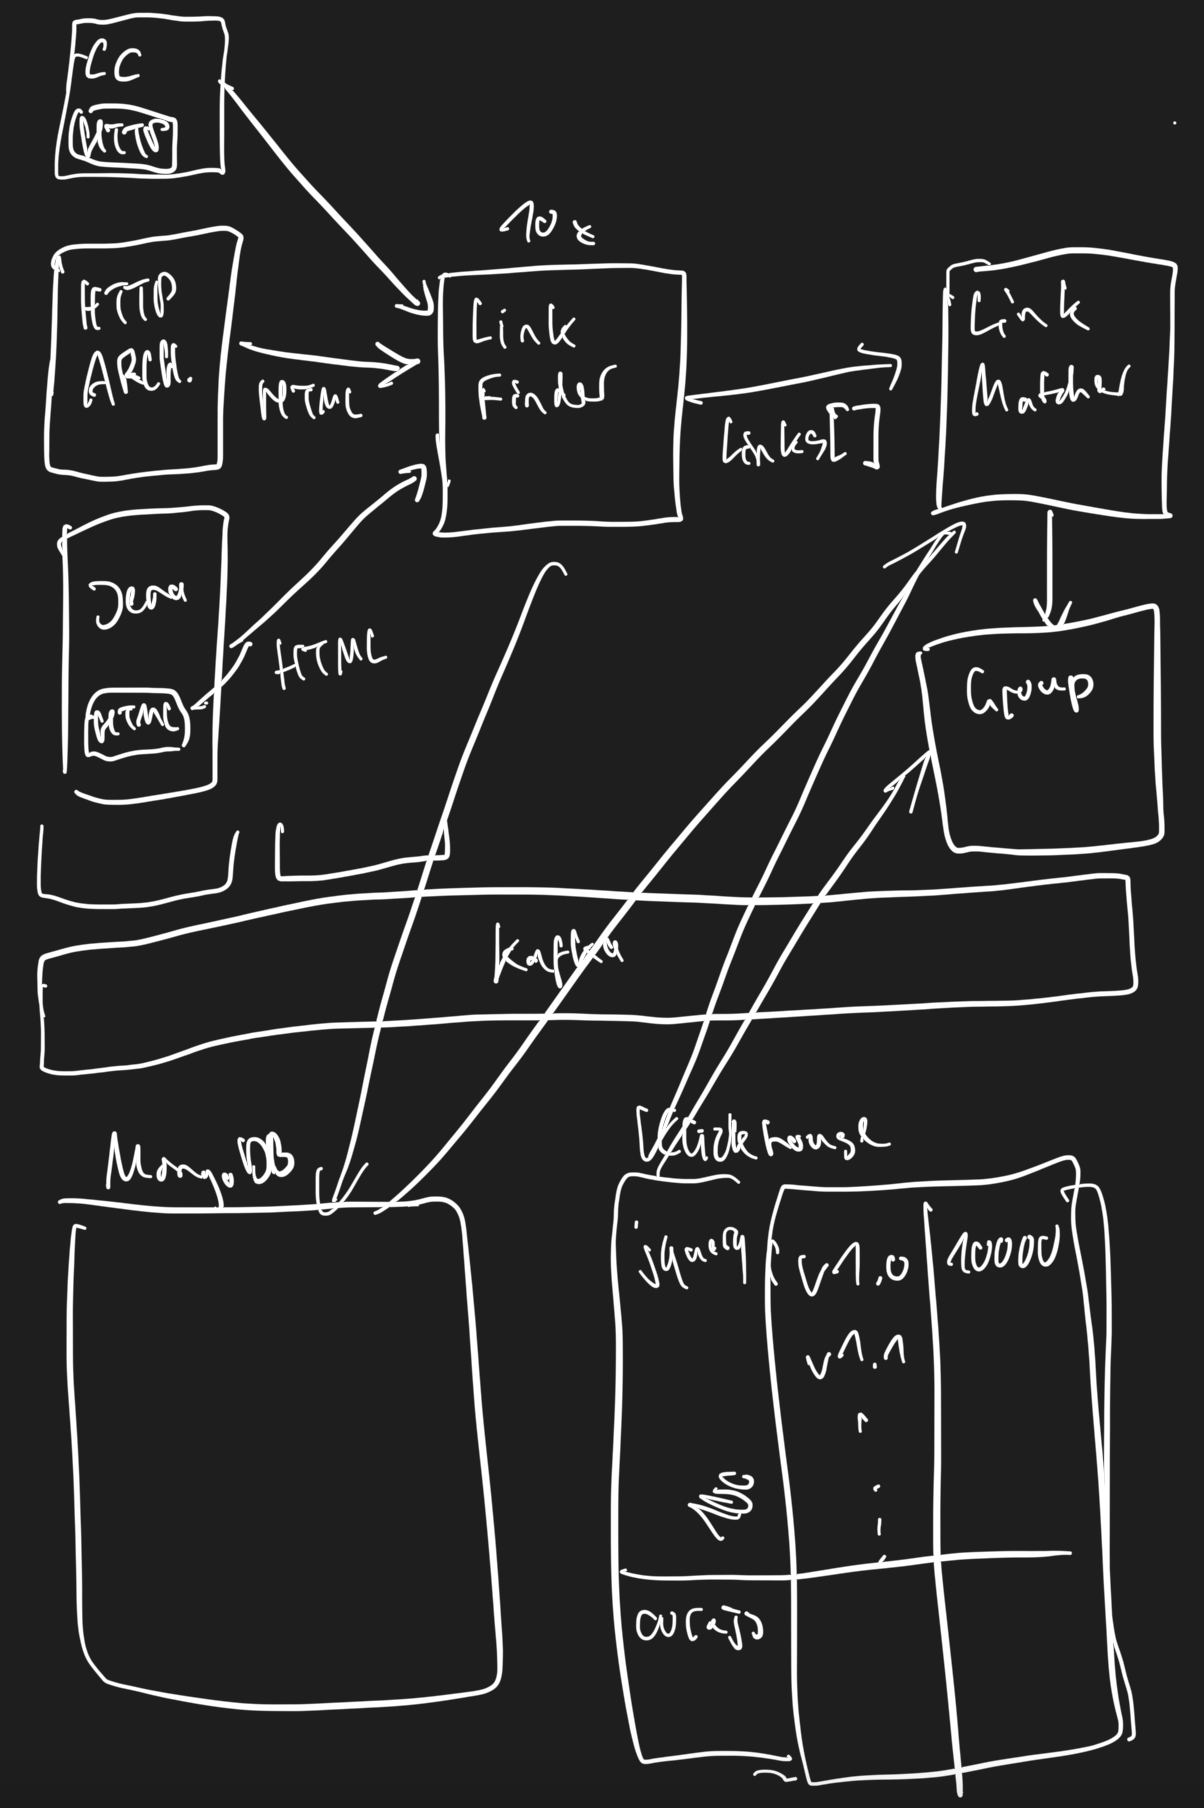
\includegraphics[width=\linewidth]{figures/approach-services.png}
      \caption{The pipeline's service architecture.}
      \label{fig:design-intuitive-approach-services}
    \end{subfigure}
    \hspace{0.05\textwidth}
    \begin{subfigure}{0.45\textwidth}
      \centering
      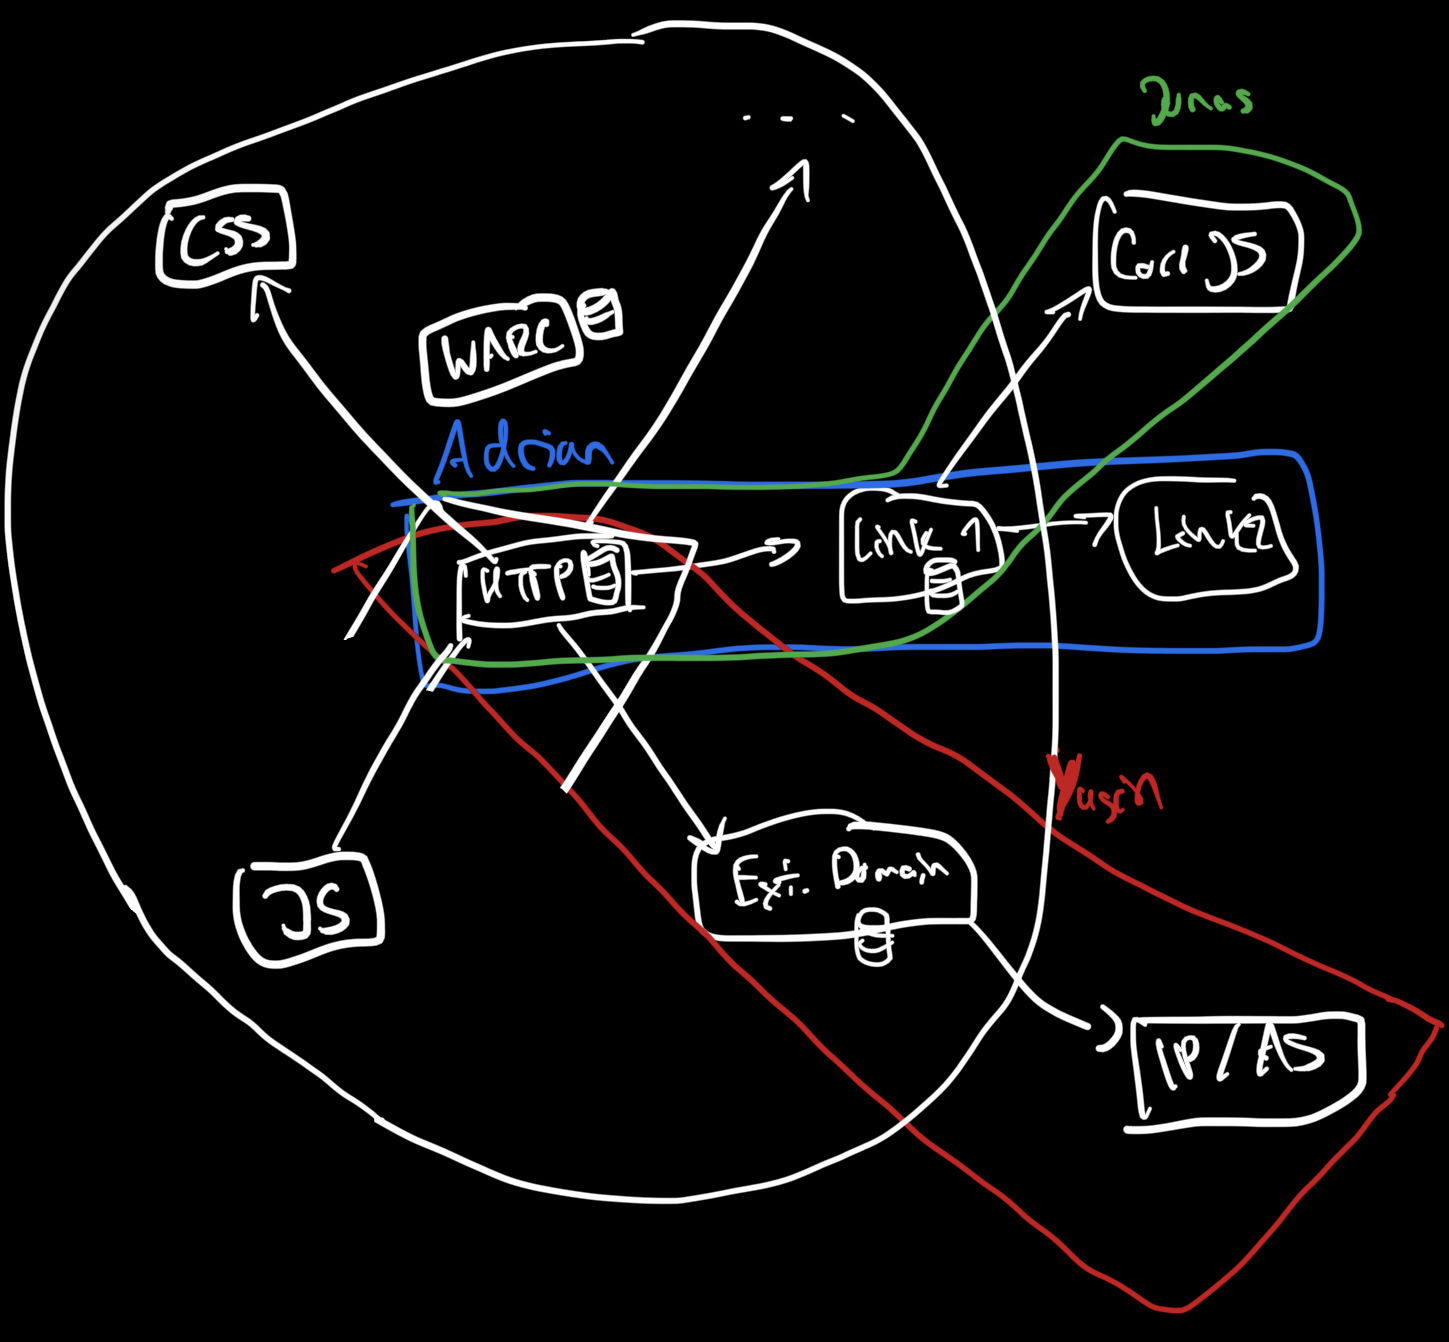
\includegraphics[width=\linewidth]{figures/approach-layered.png}
      \caption{The pipeline's data branching.}
      \label{fig:design-intuitive-approach-branching}
    \end{subfigure}
    \caption{Initial draft mockups.}
    \label{fig:design-intuitive-approach}
\end{figure}


\subsubsection{Storage}
\label{sec:design-storage}

In a distributed system, i.e., a system consisting of multiple nodes that collectively provide compute and storage resources, a key challenge is to maintain the technical guarantees of individual components when they operate within a networked environment.
A typical consumer-grade computer manages storage independently: files are saved to and retrieved from storage media directly connected to that machine.

In more complex systems with multiple nodes, a storage medium containing some data may not be physically connected to the machine requesting access to it.
Additionally, data that exceeds a single storage medium's capacity should be stored across multiple storage devices.
Storage management software, therefore, must handle reading and writing data distributed across nodes and storage media, which may only communicate via a network.

For Kubernetes, which serves as the foundational infrastructure, \href{https://longhorn.io/}{\textit{Longhorn}} provides a block storage solution.
Understanding Longhorn's distributed storage concept is fundamental, as it is the provisioned storage system in the Kubernetes cluster.

\begin{figure}[H]
    \centering
    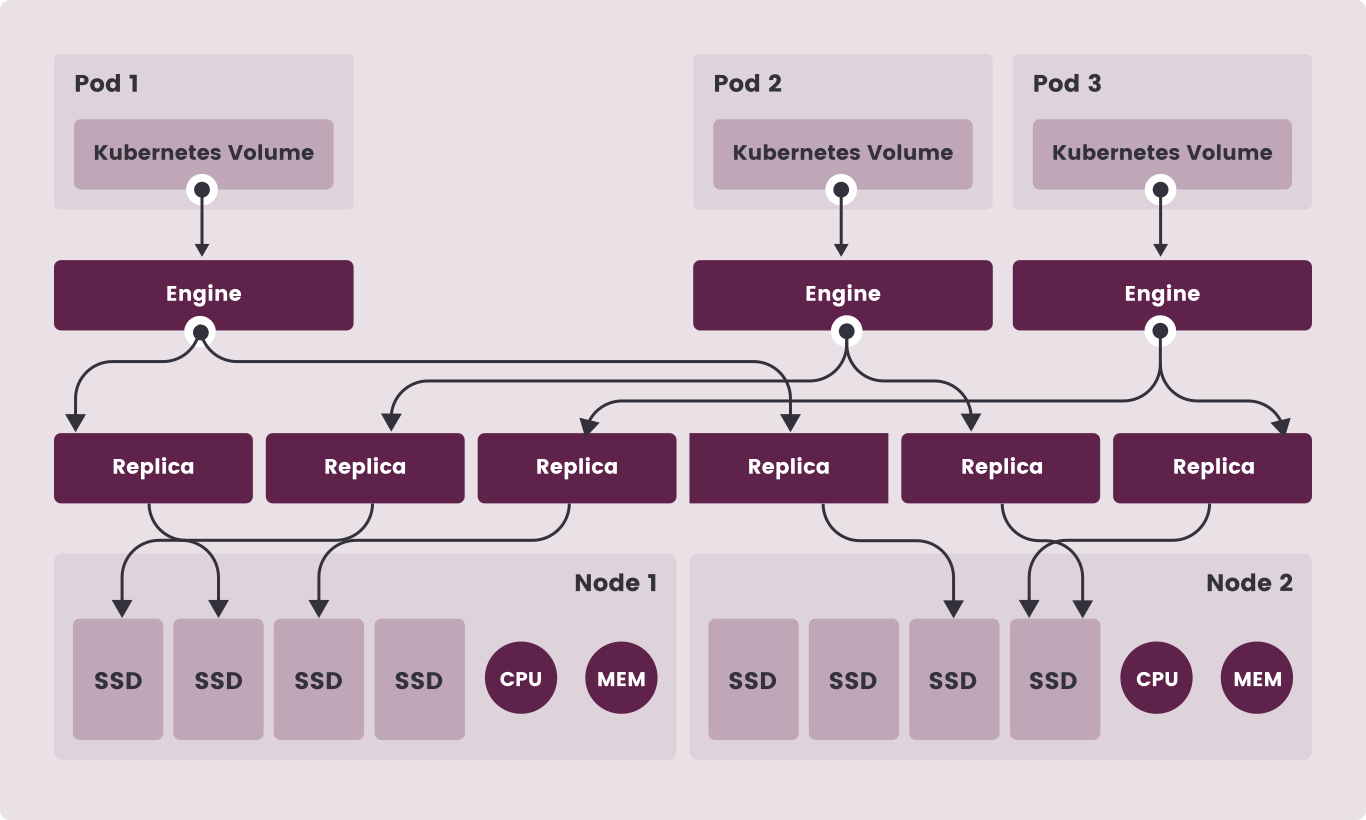
\includegraphics[width=\textwidth]{figures/longhorn.png}
    \caption{Longhorn's storage system~\cite{LonghornAuthors2024}.}
    \label{fig:longhorn}
\end{figure}

\Cref{fig:longhorn} illustrates the Longhorn storage system.
In simple terms, Longhorn enables the creation and usage of virtual storage volumes that span multiple physical storage media and nodes.
To ensure high availability and data integrity—even in the event of individual node failures—data fragments are replicated across multiple locations.
If a node fails, Longhorn automatically recreates the unavailable data replicas on other active nodes.
Longhorn also includes a snapshot-based backup functionality.

In summary, data written to Longhorn-managed storage is divided into fragments and redundantly stored across different nodes.
This fragmentation and distribution impacts the performance of computations involving the data.
If data were stored on a single distinct node, computations should ideally be conducted on a \ac{cpu} close to that node to minimize slow data transfers.
Since multiple copies of the data are spread across available nodes, however, we can generally assume that data will be accessible quickly enough\footnote{See \cref{sec:future-work-optimizations} for a potential optimization using node affinity in Kubernetes.} for computations on any node, especially considering the ease of use that Longhorn provides.

If Longhorn were not a prerequisite, it would be worth considering \acp{dfs} like \textit{Ceph}, \textit{GlusterFS}, and particularly \ac{hdfs} (the Hadoop Distributed File System).
\ac{hdfs} is a file system designed for the Hadoop project, which supports distributed computing and is promoted as a system that ``scales up from single servers to thousands of machines, each offering local computation and storage''~\cite{ASF2024b}.
Research suggests that Hadoop may be able to guarantee data locality for computational tasks.
However, placing a file system with strong data locality guarantees on top of a block storage solution with weaker guarantees, such as Longhorn, would not yield significant advantages, as the underlying system's limitations would constrain overall data locality.

In this setup, without a strict commitment to Hadoop, we retain the flexibility to choose a suitable data format, provided it is compatible with \texttt{\ac{ext4}} on a Kubernetes volume claim provisioned by Longhorn.


\subsubsection{Databases}
\label{sec:design-databases}

In the context of Big Data, \ac{olap} is more relevant than \ac{oltp} as processing large quantities of data quickly takes precedence over strict \ac{acid} guarantees.
\ac{olap} systems often use a columnar storage format, which allows for distributed execution of aggregate functions, such as calculating the minimum, maximum, average, or sum of a large dataset's numeric property.

Consider a table like \cref{tab:result-example} that stores millions of website \acp{url}, each with a country assignment and detected technologies.
For example, we might want to find the average number of web technologies used.
In a row-oriented \ac{oltp} database, each row would need to be loaded and scanned for the \texttt{web\_technology\_count} value, often passing over irrelevant columns.

\begin{table}[H]
    \centering
    \begin{tabular}{|c|c|c|c|c|}
    \hline
    \textbf{url} & \textbf{country} & \textbf{web\_technologies} & \textbf{web\_technology\_count} & \textbf{…} \\
    \hline
    https://example.jp & Japan & AMP, Google Analytics & 2 & … \\
    \hline
    \end{tabular}
    \caption{Row-oriented storage format in an OLTP system.}
    \label{tab:result-example}
\end{table}

In a columnar \ac{olap} database, values of interest can be loaded as a distinct dataset, as shown in \cref{tab:olap-example}, which allows for efficient aggregate calculations.
Here, the average of the \texttt{web\_technology\_count} is \texttt{1}.

\begin{table}[H]
    \centering
    \begin{tabular}{|c|}
    \hline
    \textbf{web\_technology\_count} \\
    \hline
    2 \\
    \hline
    0 \\
    \hline
    1 \\
    \hline
    … \\
    \hline
    \end{tabular}
    \caption{Column-oriented storage format in an OLAP system.}
    \label{tab:olap-example}
\end{table}

Another benefit of columnar storage is the potential for compression due to repetitive data patterns.
\Cref{tab:compression-example} shows an example where data, as queried on the left, could be stored more efficiently in compressed form on the right.
In simple terms, column serialization can store a value once and remember where to repeat it instead of duplicating the value.
For instance, adding a \texttt{dataset\_id} column to \cref{tab:result-example} where every record holds the same value (e.g., \texttt{CC-MAIN-2024-42}) would require minimal storage due to compression.

\begin{table}[H]
    \centering
    \begin{tabular}{|c|}
    \hline
    \textbf{country} \\
    \hline
    Germany \\
    \hline
    Germany \\
    \hline
    Germany \\
    \hline
    … \\
    \hline
    \end{tabular}
    \begin{tabular}{|c|}
    \hline
    \textbf{country} \\
    \hline
    Germany*3 \\
    \hline
    \\
    \hline
    \\
    \hline
    … \\
    \hline
    \end{tabular}
    \caption{Simplified example of view (left) and compression (right) in columnar storage.}
    \label{tab:compression-example}
\end{table}

An in-memory representation of such a columnar format is provided by \textit{Apache Arrow}, enabling support for \ac{simd} operations in modern processors.
Arrow aims to create a standard across databases and programming languages, enhancing interoperability and minimizing the need for custom serializations.
Systems such as the distributed compute engine Spark, the \ac{olap} \ac{dbms} ClickHouse, and dataframe libraries like Pandas and Polars, as well as the Apache Parquet file format, use Arrow.

An optional prerequisite in the \ac{olap} context is ClickHouse, as an instance of this solution is already provisioned in the university's Kubernetes cluster.
The \href{https://altinity.com/kubernetes-operator/}{\textit{Altinity Kubernetes Operator for ClickHouse}} simplifies the management of ClickHouse installations on Kubernetes.
However, as noted by Zhang and Dai, ClickHouse's strong coupling of storage and compute nodes poses risks to cluster stability~\cite{Zhang2023}.

ClickHouse uses the \ac{osi}-approved \textit{Apache License 2.0} open source license and is optimized for real-time analytics.
It is important to note that data freshly inserted into ClickHouse might not be immediately available for queries due to insert buffering and background merging for data compaction, as ClickHouse prioritizes fast query execution over strict data consistency.

Although real-time capabilities are out of scope for our Big Data pipeline design, ClickHouse provides an informative benchmark for analytical \acp{dbms} called \href{https://benchmark.clickhouse.com/}{\textit{ClickBench}}.
This benchmark evaluates the performance of 42 queries across 69 database systems (or configurations) on various machine or cluster sizes.
Metrics for data load time, storage size, as well as cold and hot run performance, are also provided for comparison.

For this thesis, the following \ac{olap} systems were selected for closer inspection based on an extensive search for popular solutions: ClickHouse, \href{https://doris.apache.org/}{\textit{Apache Doris}}, \href{https://druid.apache.org/}{\textit{Apache Druid}}, \href{https://pinot.apache.org/}{\textit{Apache Pinot}}, and \href{https://starrocks.io/}{\textit{StarRocks}}.
Additional noteworthy mentions include:

\begin{itemize}
    \item \href{https://snowflake.com/}{\textbf{Snowflake}}, which achieves minimal storage size but is only available as a hosted cloud service with credit-based pricing, based on virtual warehouse size and hours of compute;
    \item \href{https://clickhouse.com/chdb}{\textbf{chDB}} and \href{https://duckdb.org/}{\textbf{DuckDB}}, which function as in-process engines similar to what \href{https://www.sqlite.org/}{\textit{SQLite}} offers for \ac{oltp};
    \item \href{https://motherduck.com/}{\textbf{MotherDuck}}, a hosted cloud service for DuckDB; and
    \item \href{https://postgresql.org/}{\textbf{PostgreSQL}} as a performance reference for an \ac{oltp} \ac{dbms}: PostgreSQL requires approximately 88 times the load time, 50 times the hot and cold run times, and ten times the storage size compared to each category's baseline.
\end{itemize}

ClickBench highlights individual challenges faced by Pinot and Druid.
For Pinot, the following observations are made:

\begin{quote}
    ``It successfully loaded only 94465149 out of 99997497 records.
    Some queries returned NullPointerException.
    The loading process is painful - splitting to 100 pieces required.
    It does not correctly report errors on data loading, the results may be incorrect.''~\cite{Milovidov2022}
\end{quote}

For Druid:

\begin{quote}
    ``Druid is killed and restarted after every query.
    Otherwise some queries make Druid degraded and results are incorrect.
    For example after Q13 even SELECT 1 works for 7 seconds.''~\cite{Milovidov2022}
\end{quote}

These observations, documented by Alexey Milovidov, led to the decision to exclude Pinot and Druid as database systems for the Big Data pipeline designed here.

This leaves us with Apache Doris and StarRocks.
Doris is notable for its straightforward architecture.
In contrast, Pinot and Druid rely on \textit{Apache Zookeeper} for service coordination, with Druid, in particular, requiring a complex architecture involving a coordinator, overlord, broker, historical, and middle manager services.
Doris, on the other hand, only requires frontend services for query planning, backend services for data execution, and a meta store for metadata management.

StarRocks is a fork of Doris, with licensing and trademarking challenges arising between the projects after the fork~\cite{Chen2024}.
Originally named \textit{DorisDB}, StarRocks initially used the \textit{Elastic License}, which disqualified it from open source designation due to restrictions on commercial use.
In 2022, however, StarRocks switched back to the Apache License 2.0, the same license Doris uses.
Both Doris and StarRocks support the Lakehouse architecture and the Iceberg table format.

Before discussing distributed computing, it is worth outlining another use case for querying: querying across multiple heterogeneous data sources.
Data systems that evolve over time often amass multiple data pools.
For instance, some data may be stored in an \ac{oltp} \ac{dbms} like PostgreSQL, while other data might reside in a cloud data warehouse like Snowflake or similar alternatives.
This chapter ultimately selects a storage solution as a design choice, which may complement existing data stores at the academic institution.
To integrate this data and make the results of this thesis available for future research, a system capable of querying across diverse sources is essential.
This is where \textit{Trino} becomes relevant.

Trino is a fork of a project commonly known as \textit{Presto}, originally developed at Facebook.
Similar to the StarRocks fork from Doris, there was some ambiguity around the ownership of \textit{PrestoSQL} (the rebranded fork) and \textit{PrestoDB} (the original project).
The name change to Trino resolved this issue~\cite{Traverso2022}.

However, the databases and query engines mentioned are unsuitable for the flexible transformations we aim to enable in our Big Data pipeline.
Beyond merely reading table results, it should be possible to perform arbitrary computations on the data and insert results back into the dataset.
Thus, a proper design for data computations must be defined.

\subsection{Envisioned Result}
\label{sec:design-envisioned-result}

The final output of our Big Data pipeline should be clear visual insights that simplify understanding a large dataset.
Since we are working with global data, choropleth maps provide an effective visualization format.
Choropleth maps display a geographic area in which regions are shaded according to a statistical value.
These maps are often used to present election results, with sub-areas shaded in the winning party's color.

\Cref{fig:choropleth} illustrates a choropleth map that could represent the output of the Big Data pipeline designed in this thesis.
It shows a world map with countries shaded based on a metric such as the number of websites attributed to each country.
The map could display the total number of websites processed, websites above a certain size, or websites containing specific technology, such as the \textit{Wordpress} blogging platform.
Choropleth maps also help identify potential data biases; for instance, if many countries in a continent like Africa are left unshaded, the dataset may contain a bias warranting further investigation.

\begin{figure}[H]
    \centering
    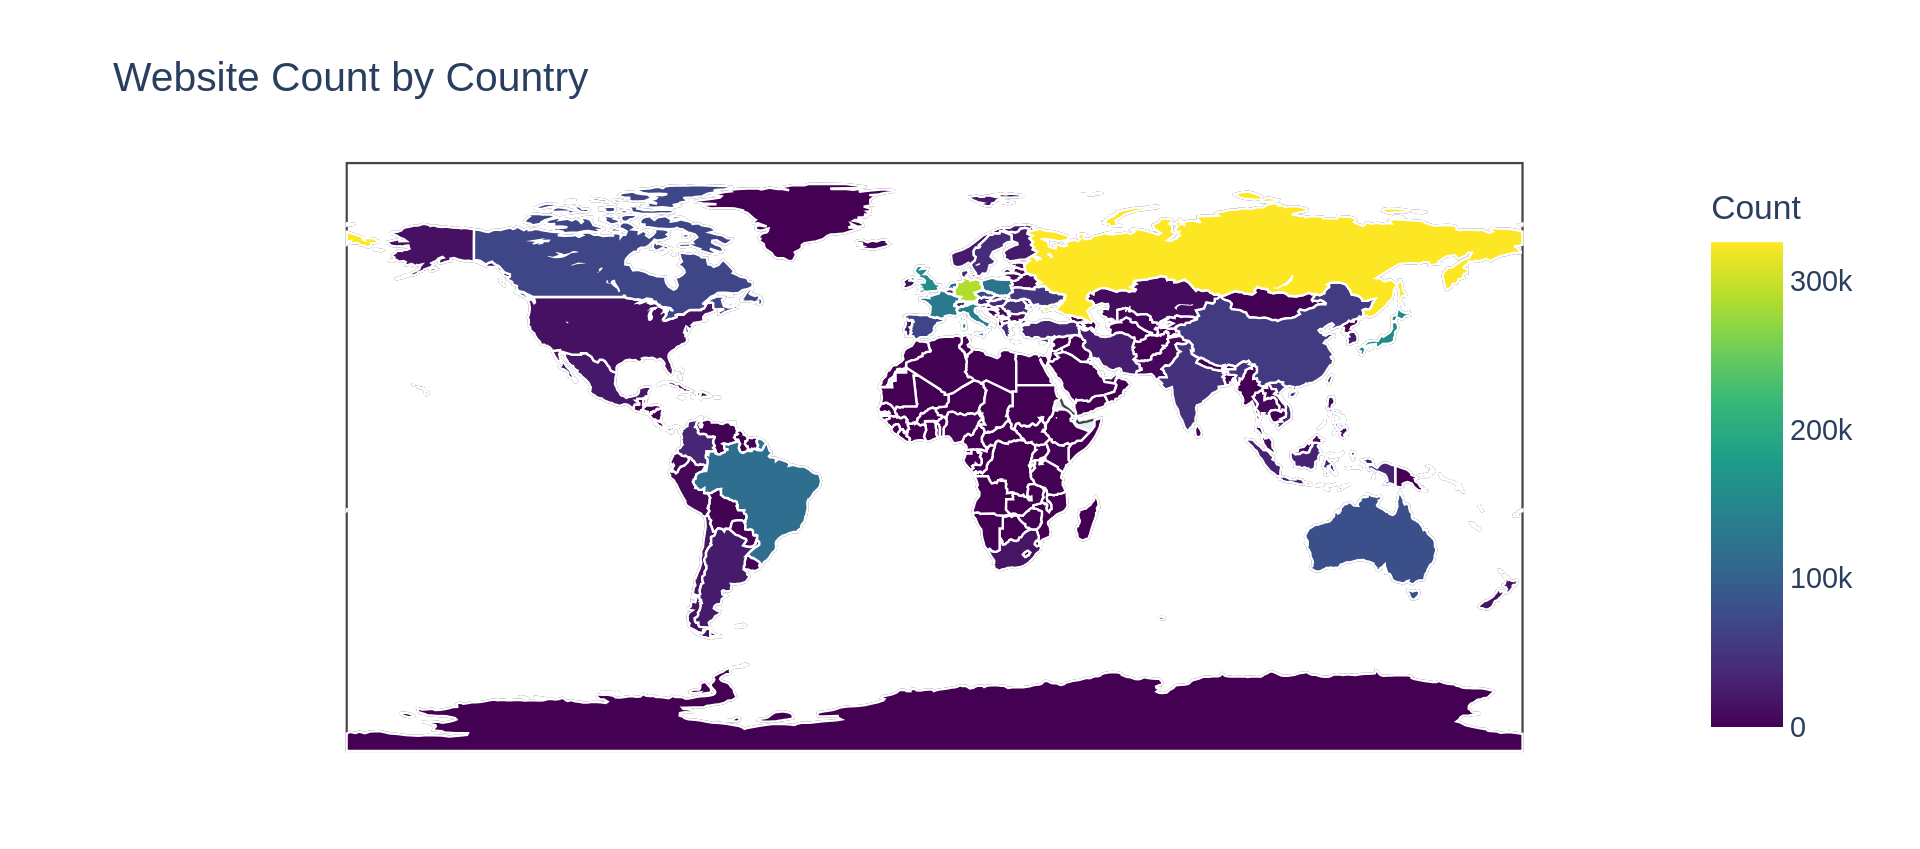
\includegraphics[width=\textwidth]{figures/charts/large/chart_fact_uri_choropleth.png}
    \caption{An example choropleth map showing the number of websites per country.}
    \label{fig:choropleth}
\end{figure}

The first design decision necessary is to determine how to attribute websites to specific countries.
Possible options include using the IP address of the website's host server, the address of a domain's owner, or the language of the text visible to website visitors.
However, because our top-down approach has delayed dataset selection, we are not yet certain which of these data types will be readily available.
Therefore, we choose to use part of a metric that is likely to be consistently accessible: a website's \ac{cctld}, such as \texttt{.de} in \texttt{https://example.de/page}.

A website's \ac{cctld} does not guarantee that its content is intended for citizens of the corresponding country or that it was created by residents of that country.
For example, \texttt{https://\-maev.si/} uses Slovenia's \ac{cctld} purely for a wordplay effect, while targeting German users.
Nevertheless, using the \ac{cctld} is sufficient for evaluating the capabilities of the Big Data pipeline.

Before proceeding to the next step, it is essential to remember that choropleth maps represent just one option for displaying results and should not restrict alternative methods of data interpretation.

Data visualization tools vary in their target user groups and feature sets.
Microsoft's \href{https://microsoft.com/power-platform/products/power-bi}{\textit{Power BI}} and Salesforce's \href{https://tableau.com/}{\textit{Tableau}} are designed primarily for corporate use cases.
These solutions are hosted by their providers, eliminating setup and maintenance costs for running the software on internal infrastructure.
However, as a result, these products are commercial offerings.
Both providers offer discounts for students and academic institutions.

Since internal infrastructure is already in place, as discussed in \cref{sec:design-prerequisites}, a lightweight alternative could be used to avoid dependency on external providers.

Open source solutions for data visualization include \href{https://superset.apache.org/}{\textit{Superset}} by the Apache Software Foundation and \href{https://redash.io/}{\textit{Redash}}, a community-driven project.
All of the tools mentioned so far enable the definition of connections to data sources, execution of queries against those data sources, and creation of dashboards that visually compose the results of these queries.
\Cref{fig:superset-dashboard} shows an example of a Superset dashboard, while \cref{fig:redash-query-editor} provides an example of the Redash query editor.

The main takeaway is that these tools offer interactivity, allowing visualizations to be defined and modified at runtime.
This feature-rich environment is beneficial for end users of data pipelines, such as data scientists.
However, this level of functionality also introduces complexity: for instance, Superset requires at least a metadata database, and for certain features, it also relies on a caching layer as well as a worker and beat service~\cite{ASF2024}.
This additional infrastructure is excessive for the non-essential part of the data pipeline design, especially since the visualization tools' data source support could become a limiting factor in upcoming storage decisions.
Nonetheless, it is important to be aware of these feature-rich solutions, as a solid data pipeline implementation could integrate these tools in future extensions.


\subsection{Decisions}
\label{sec:design-decisions}

Now that \cref{sec:design-prerequisites} has defined the prerequisites and \cref{sec:design-envisioned-result} has outlined our goal, we are able to make the necessary decisions to design the Big Data pipeline that meets the objectives defined in \cref{sec:intro-objectives}.
With Longhorn set as the storage solution, our first decision is to select a tool that enables complex distributed computations.
We then review our findings from \cref{sec:related-work-big-data-pipelines} on the characteristics of a modern Big Data pipeline and select a storage layout that fits our requirements.
With these two decisions in place, and with priority given to compatibility, flexibility, and popularity, the choice of programming language becomes straightforward.

These three foundational choices enable the systematic design of a data architecture within storage.
Finally, a modern \ac{gui} for managing workflows is selected.


\subsubsection{Compute}
\label{sec:design-compute}

As noted in \cref{sec:design-databases}, our dataset requires transformational computations that extend beyond simple querying.
For this purpose, the batch processing engine Spark offers a well-established and powerful open source framework for \ac{mpp}.
Spark's stream processing counterpart is Flink, although Spark also supports streaming in a limited form through micro-batching.
Flink graduated from Apache's incubation at the end of 2014, shortly after Spark completed its own graduation in February of the same year.

At its core, Spark utilizes \acp{rdd} for fault-tolerant distribution of immutable objects across a cluster's nodes without requiring redundant copies.
This approach is known as lineage-based fault tolerance.
If a partition of an \ac{rdd} is lost, Spark can recover it by tracing the lineage of transformations that created it.

In Scala and Java, these distributed objects can be manipulated via Spark's \textit{Dataset API}.
In Python and R, the \textit{DataFrame API} provides a similar structure, offering a dataset accessible through named columns.
The DataFrame API is also available in a row-based format for Scala and Java.
These \acp{api} provide comfortable abstractions for direct interaction with \acp{rdd}.

Spark performs computations in-memory, distinguishing it from disk-based processing frameworks like Hadoop, which executes the MapReduce model and writes results back to disk, generally making it slower than in-memory processing.

In the Hadoop MapReduce context, querying is facilitated by \href{https://hive.apache.org/}{\textit{Apache Hive}}, whereas Spark provides \textit{Spark SQL} as its native querying module, which also supports reading from Hive installations.

Other Spark modules include the \ac{ml} library \textit{MLlib} and \textit{GraphX}, an \ac{api} for graph-based computations.
Although these modules are not utilized in this thesis, they may be beneficial for future extensions.

A distributed Spark job involves three primary components:

\begin{itemize}
    \item \textbf{Drivers}, which initiate the software.
    \item \textbf{A master}, coordinating the executors.
    \item \textbf{Executors}, which handle their allocated portions of a job.
\end{itemize}

Spark can be deployed in either \textit{Client Mode} or \textit{Cluster Mode}.
In Client Mode, the Driver runs on the client machine that submits the job and must remain connected to the cluster to maintain the connection.
In Cluster Mode, the Driver operates on a worker node within the cluster, allowing the client to disconnect without impacting the job's execution.
\Cref{fig:spark-cluster} illustrates Spark's Cluster Mode, where Kubernetes, \href{https://mesos.apache.org/}{\textit{Apache Mesos}}, and \href{https://hadoop.apache.org/docs/current/hadoop-yarn/hadoop-yarn-site/YARN.html}{\textit{Apache Hadoop YARN}} are possible cluster managers.

\begin{figure}[H]
    \centering
    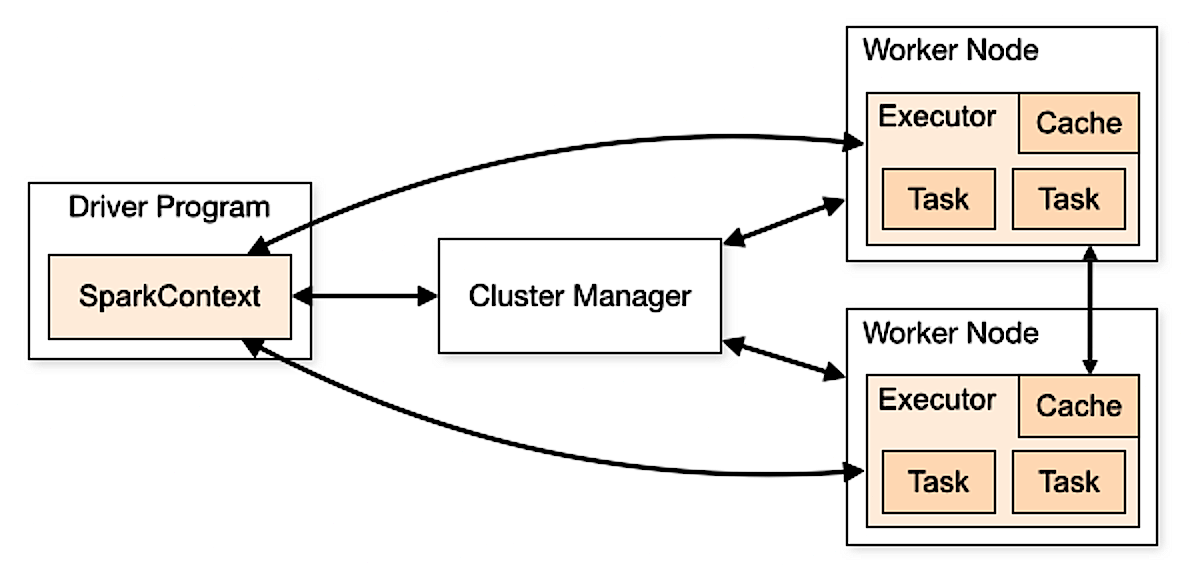
\includegraphics[width=0.75\textwidth]{figures/spark-cluster.png}
    \caption{Spark's architecture in cluster mode~\cite{ASF2024c}.}
    \label{fig:spark-cluster}
\end{figure}


\subsubsection{Data Format}
\label{sec:design-decisions-data-format}

We select an open table format because, with Spark as our distributed compute and query engine, we are not restricted to any format specific to a particular data management tool.
This decoupling aligns with the Lakehouse architecture.

There are three primary options for open table formats supporting the Lakehouse architecture:

\begin{itemize}
    \item \href{https://delta.io/}{\textit{\textbf{Delta Lake}}}, open-sourced in 2019 as part of the \href{https://www.databricks.com/}{\textit{Databricks}} ecosystem, later joined the Linux Foundation in 2020, reflecting a commitment to open governance and broader community development.
    \item \href{https://iceberg.apache.org/}{\textit{\textbf{Apache Iceberg}}}, open-sourced by \href{https://www.netflix.com/}{\textit{Netflix}} in 2018, was donated to the Apache Software Foundation in 2019, achieving top-level project status in 2020.
    \item \href{https://hudi.apache.org/}{\textit{\textbf{Apache Hudi}}}, open-sourced by \href{https://www.uber.com/}{\textit{Uber}} in 2017, became an Apache Incubator project in January 2019 and graduated to top-level project status in May 2020.
\end{itemize}

These tools vary in aspects such as Hudi's write optimization or external support, e.g., Iceberg is supported by Snowflake, whereas Hudi is not.
Fortunately, efforts have been made to simplify switching between formats or even using multiple formats simultaneously.
This flexibility is achieved by separating data files from metadata files.
Tools like \href{https://xtable.incubator.apache.org/}{\textit{Apache XTable}}\footnote{XTable was formerly known as \textit{OneTable} and was created by \href{https://www.onehouse.ai/}{\textit{Onehouse}}, a Lakehouse cloud provider.} and \href{https://www.databricks.com/product/delta-lake-on-databricks}{Delta Lake UniForm} convert metadata files across table formats while leaving data files unchanged.
However, certain tool-specific strengths, such as Hudi's write performance, may not be fully retained if Delta Lake is used as the foundation~\cite{Merced2024}.
An emerging real-time format for the Lakehouse architecture is \href{https://paimon.apache.org/}{\textit{Apache Paimon}}, though it is not yet as widely adopted as the previously mentioned solutions.

Another noteworthy tool is \href{https://projectnessie.org/}{\textit{Nessie}}, introduced by \href{https://www.dremio.com/}{\textit{Dremio}}.
Nessie, a transactional catalog, provides Git-like version control features for Iceberg Lakehouse storage.
With Nessie, it is possible to commit data changes transactionally across multiple branches without copying data.
This capability enables navigation through data history and parallel data versions, which was identified as a goal in \cref{sec:design-prerequisites-intuitive-approach} and illustrated in \cref{fig:design-intuitive-approach-branching}.
While Nessie will not be used in this thesis, researching it provided valuable insights into Iceberg, leading to the decision to use Iceberg as the open table format for the upcoming implementation.


\subsubsection{Programming Language}
\label{sec:design-decisions-programming-language}

The initial rationale for selecting TypeScript as the programming language for the Big Data pipeline, as outlined in \cref{sec:design-prerequisites-intuitive-approach}, was that those interested in website data analysis typically have experience in web development and are accustomed to TypeScript.
However, the research into Big Data, data engineering, and data science covered in \cref{sec:related-work-big-data}, along with the analysis of tools that best meet the targeted capabilities of the pipeline, points toward Python as the more suitable choice.

The design of a Big Data pipeline falls squarely within data engineering.
The primary objective of this thesis is to support future researchers by providing well-justified choices for tools that meet the goals defined in \cref{sec:intro-objectives}.
Specifically, the pipeline aims to assist researchers in exploring novel datasets and advancing scientific insights.
It is therefore essential to choose a programming language that offers robust integration within the data engineering ecosystem to avoid compatibility limitations and maintain flexibility in scientific applications.
This requirement suggests selecting a language that is both popular and extensively supported within the data engineering domain.

Python is a leading programming language across data engineering, data science, and artificial intelligence, and it ranked as the most popular language among coding learners in the 2024 \textit{Stack Overflow} developer survey~\cite{StackExchange2024}.
Python is also taught at the academic institution hosting this research.
Thus, selecting Python as the language for the Big Data pipeline will ensure broad accessibility for developers who will work with, extend, or integrate the system.

As discussed in \cref{sec:design-compute}, Spark provides a straightforward means of distributed computation for the pipeline's transformation stage.
Through \textit{PySpark}, it is easy to initiate Spark jobs in Python, offering strong alignment with the Python ecosystem.

TypeScript is also widely used, especially in web development, but it is less common in data-centric engineering fields.
TypeScript adds typing to \textit{ECMAScript} (commonly known as \ac{js}) and can be executed in environments like \href{https://nodejs.org/}{\textit{Node.js}}, \href{https://deno.com/}{\textit{Deno}}, or \href{https://bun.sh/}{\textit{Bun}}.
The main package ecosystem for \textit{ECMAScript} is the \href{https://www.npmjs.com/}{\textit{npm}} registry.
However, no actively maintained Spark client comparable to PySpark for Python could be found in npm.

Thanks to \textit{Apache Livy}, a \ac{rest} \ac{api} can be set up for Spark, enabling interaction with Spark from any language that supports \ac{http} requests.
Without Livy, establishing a Java socket server to act as middleware between the client and Spark would be necessary, along with a custom client implementation.
Nevertheless, the most widely documented method of interacting with Spark remains PySpark, further supporting Python as the optimal choice.


\subsubsection{\ac{elt}}
\label{sec:design-decisions-elt}

As shown in \cref{sec:related-work-big-data-pipelines}, a modern storage environment like Rancher allows for using the \ac{elt} step order instead of the \ac{etl} order in our pipeline.
This section explains our decisions on how extraction, loading, and transformation will be implemented.

With Python as the programming language of choice, we have the flexibility to define connectors to various sources from which we wish to extract data.
Data movement tools like \href{https://www.fivetran.com/}{\textit{Fivetran}} or \href{https://airbyte.com/}{\textit{Airbyte}} offer standalone alternatives with predefined connectors configurable via a \ac{gui} and support for custom connectors.
However, choosing a separate data movement tool would result in tool-specific configurations, which would be less flexible to migrate to alternatives than Python source code, as Python is one of the most popular programming languages, as discussed in \cref{sec:design-decisions-programming-language}.

The \textit{Medallion Architecture} is a logical data structure for Lakehouses, depicted in \cref{fig:design-decisions-elt-medallion}~\cite{Emilio}.
Data extracted from sources is first loaded as-is into a ``bronze'' storage layer.
Since such raw data often does not meet expected quality standards, transformations that ensure quality requirements are met store their results in a ``silver'' storage layer.
An intuitive example of a data quality improvement is the transformation of numerical values provided as strings by the data source into integers.
The final ``gold'' storage layer can be understood as a warehouse representation.
In Iceberg, we designate the database representing the bronze layer as \texttt{raw}, the silver layer as \texttt{staging}, and the gold layer as \texttt{marts}\footnote{In Iceberg database and namespace are synonymous.}.

\begin{figure}[H]
    \centering
    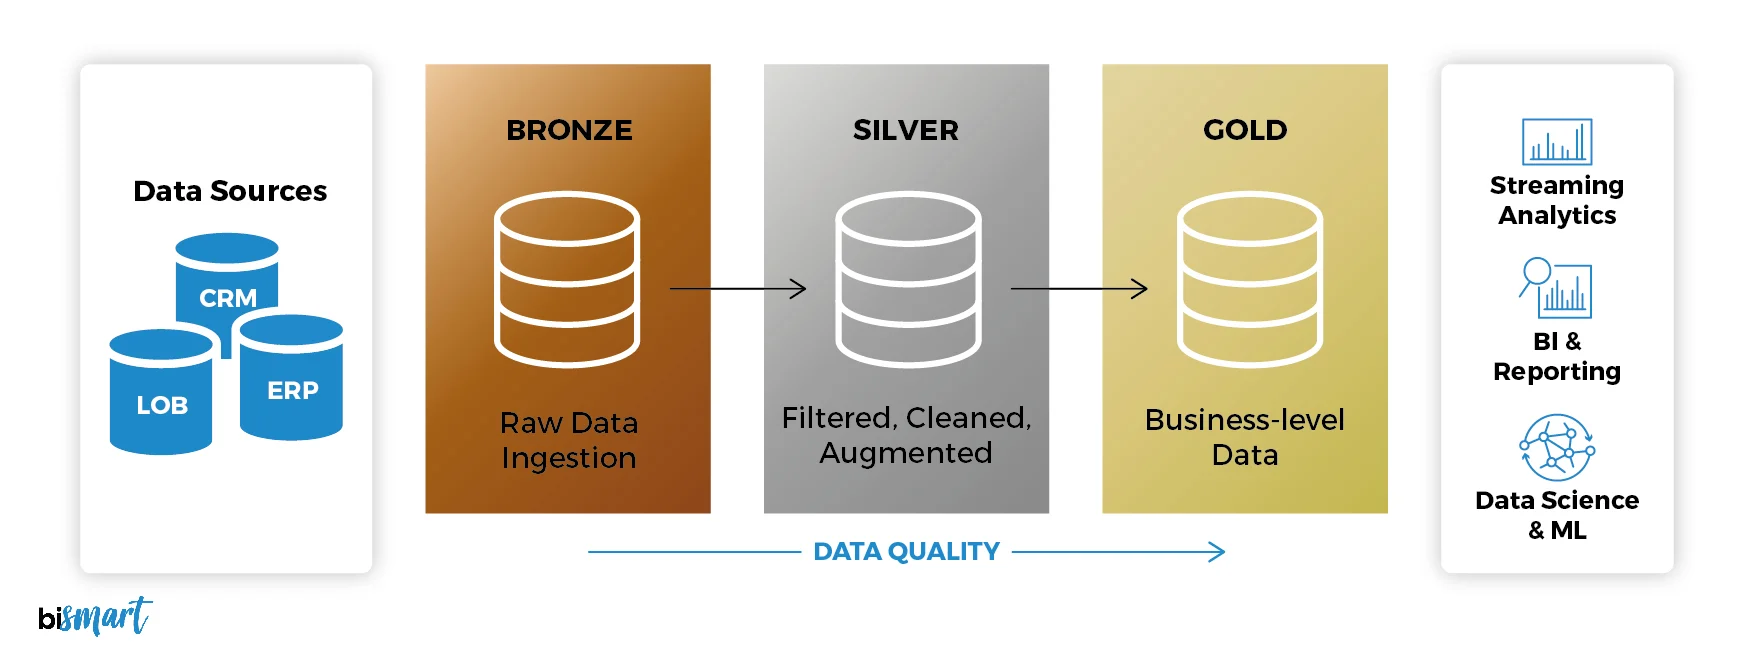
\includegraphics[width=\textwidth]{figures/medallion.png}
    \caption{Medallion architecture for the Lakehouse~\cite{Emilio}.}
    \label{fig:design-decisions-elt-medallion}
\end{figure}

The transformations we plan to implement can be categorized into two types: \ac{sql}-type transformations, which can be fully executed using \ac{sql} statements, and script-type transformations, which require functionality beyond the expressiveness of \ac{sql} (e.g., the functionality of a programming language like Python).
Especially the clean-up transformations between the bronze and silver layers can generally be covered by \ac{sql}-type transformations.

A tool specifically built for efficiently managing \ac{sql}-type transformations for a project is \href{https://www.getdbt.com/}{\textit{dbt}}.
dbt allows us to define \ac{sql} statements in a modular and interconnected manner to ensure data source integrity.
dbt modules are centered around \acp{cte} and feature a dependency mechanism through which different \ac{sql} scripts build on one another.
Additionally, dbt modules can be documented, versioned, tested, and deployed to production.
In this way, dbt serves as the central tool for \ac{sql}-type transformations and becomes more valuable as the number of \ac{sql} statements managed by it increases.

To benefit from the consistently structured handling of \ac{sql} transformations, which we expect to need at least once for each data source between the bronze and silver layers, we choose to adopt dbt early instead of using plain \ac{sql} strings in Python.
The amount of transformations needed between the silver and gold layers is expected to be minimal for now but will likely grow with each additional use case for the available data.


\subsubsection{Workflow Orchestration}
\label{sec:design-decisions-orchestration}

In the previous section, \cref{sec:design-decisions-elt}, we concluded that there are two types of transformations, with only one type covered by dbt.
The script-type transformations are instead to be defined in Python.
Also, our pipeline requires a \ac{gui} to allow for graphical interactions and intuitive insights.

\href{https://dagster.io/}{\textit{Dagster}} is a visual workflow orchestration tool that allows both types of transformations to run, thereby completing our pipeline.
In Dagster, Python functions decorated with \texttt{@asset} appear on the \ac{gui} as workflow elements.
Dagster assets can have dependencies and can therefore form a \ac{dag}, as shown in \cref{fig:design-decisions-orchestration-asset}.

\begin{figure}[H]
    \centering
    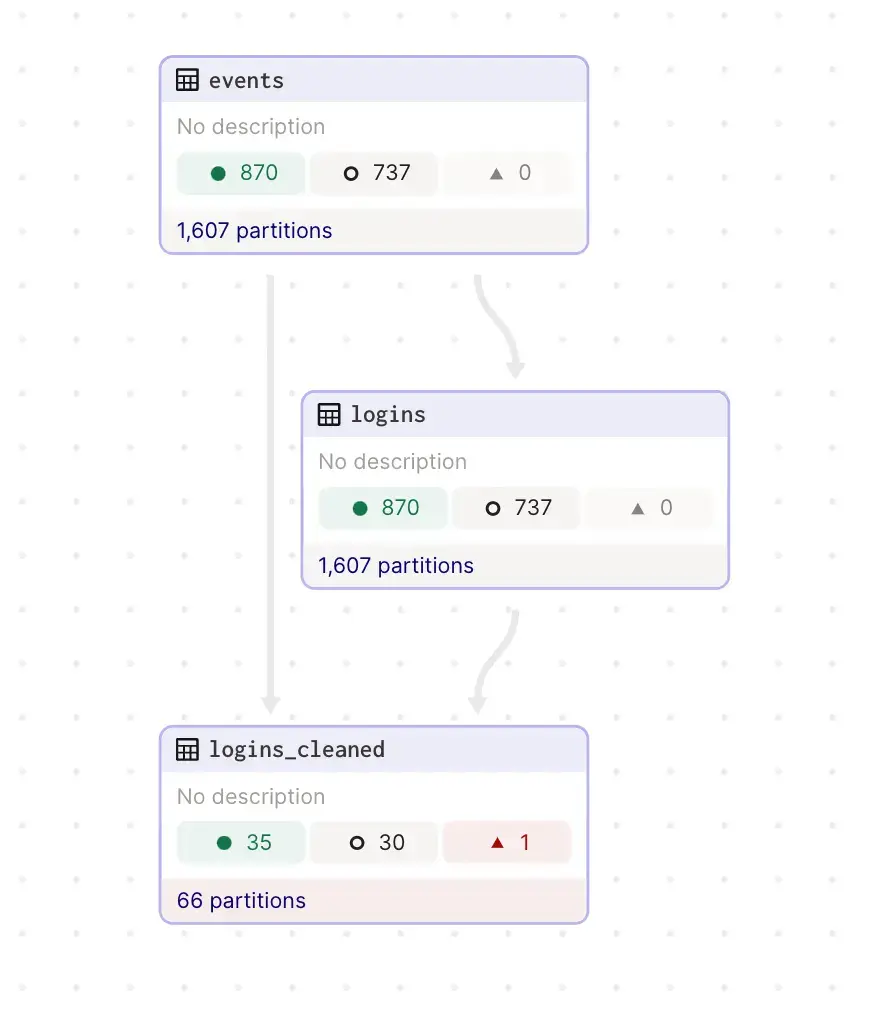
\includegraphics[width=0.6\textwidth]{figures/dagster-partitioned-asset-graph.png}
    \caption{Example of three partitioned Dagster assets forming a \ac{dag}~\cite{Ryza2023}.}
    \label{fig:design-decisions-orchestration-asset}
\end{figure}

With each Dagster asset representing a stored object, such as a table, Dagster offers first-class support for partitioning.
For instance, if hourly partitioning is used, asset runs can be scheduled and backfilled predictably, while maintaining full consistency with parent asset runs.
Alternatively to interval-based asset scheduling, Dagster also allows configuring sensors that trigger asset runs on demand.

Dagster can host multiple workflows sourced from ``code locations'', which can be Python modules or code files.
In development, code changes are loaded without the need to restart Dagster, while in production the Dagster web server can run separately from the user code.

Dagster has a native integration with dbt, mapping dbt's models to Dagster's assets, as shown in \cref{fig:design-decisions-orchestration-dbt}.
A dbt model's filename is interpreted as if it were the name of a Python function with an \texttt{@asset} decorator.
Any references in a dbt model are considered dependencies of a Dagster asset, as specified in the Python function's parameters.

\begin{figure}[H]
    \centering
    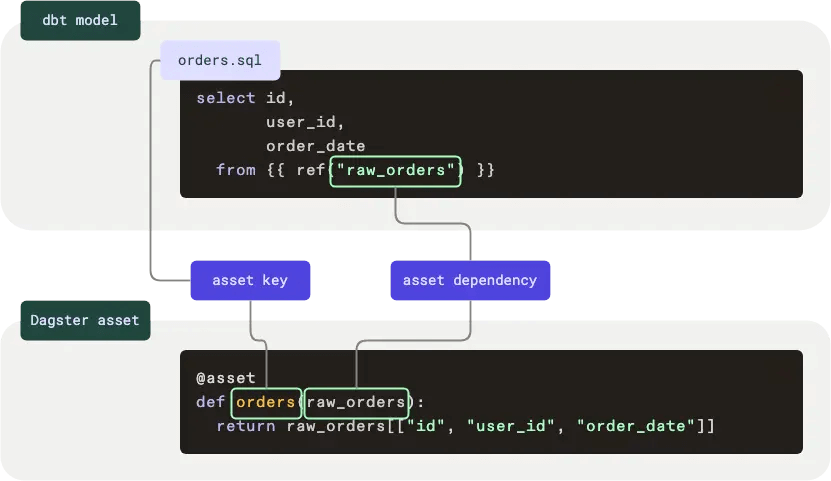
\includegraphics[width=0.8\textwidth]{figures/dagster-dbt.png}
    \caption{Comparison of dbt model and Dagster asset~\cite{DeMaria2022}.}
    \label{fig:design-decisions-orchestration-dbt}
\end{figure}

Alternatives to Dagster include Airflow and NiFi, as introduced in \cref{sec:related-work-big-data-pipelines}.
However, both Airflow and NiFi lack the native partitioning capabilities of Dagster.
Additionally, NiFi is heavily oriented towards real-time processing, emphasizing related quality-of-life features like fine-grained backpressure handling.
In our use case, we do not need to closely track each entity's movement through the system, which saves us some overhead.
Although NiFi pipelines can be configured via low-code \ac{gui} interaction, the available operators for external system interactions, such as those with Iceberg, are limited.
At the time of writing, NiFi only supports adding rows to Iceberg tables, and other interactions like table creation must be done through an external system.

Dagster appears to offer exactly the features we need to orchestrate our pipeline workflow without the limitations of Airflow and NiFi, so we decide to implement Dagster into our pipeline.
